\begin{frame}

\frametitle{Buffery}
	\begin{itemize}
		\item Buffer je paměť na GPU
		\item Unikátní celočíselný identifikátor
		\item Může být připojen na různá místa VBO, EBO, ...
		\item Několik způsobů zápisu a používání
		\item Zápis/čtení z CPU/GPU
	\end{itemize}
\end{frame}


\begin{frame}
\frametitle{Použití Buffer}
    \begin{enumerate}
        \item{Získání jména Bufferu.}
				\item{Vytvoření Bufferu}
				\item{Alokace místa pro Buffer}
				\item{Nahrání dat do Buffer}
				\item{Připojení Bufferu}
				\item{Uvolnění Buffer.}
    \end{enumerate}
\end{frame}


\begin{frame}[fragile]

\frametitle{Vytvoření/uvolnění identifikátorů}
	\begin{itemize}
		\item{Pomocí identifikátoru (jména) komunikujeme s buffery.}
		\item{
		Vytvoření identifikátorů:\\
		{\scriptsize
		\mint[frame=lines]{c++}|void glGenBuffers(GLsizei n,GLuint * buffers);|
		}
		\begin{description}
			\item[n] Počet identifikátorů (jmen), které chceme vytvořit
			\item[buffers] Pole idenifikátorů
		\end{description}
		}

		\item{
		Uvolnění identifikátorů:\\
		{\scriptsize
		\mint[frame=lines]{c++}|void glDeleteBuffers(GLsizei n,GLuint * buffers);|
		}}

		\item{
		Funkce {\color{blue}glGenBuffers} má podobnou funkcionalitu jako funkce {\color{blue}glGenTextures}.
		}
	\end{itemize}
\end{frame}

\begin{frame}
\frametitle{Připojení Bufferu k targetu}
	\begin{itemize}

		\item{ Aktivování bufferu - touto funkcí určíme buffer, se kterým budeme pracovat dany target:\\
		{\scriptsize
		\mint[frame=lines]{c++}|void glBindBuffer(GLenum target,GLuint buffer);|
		}
		\begin{description}
			\item[target] Určuje typ bufferu a způsob jeho používání.
			\item[buffer] Identifikátor (jméno) bufferu.
		\end{description}
		}

	\end{itemize}
\end{frame}

\begin{frame}
\frametitle{Připojení Bufferu k targetu}
	\begin{figure}[h]
	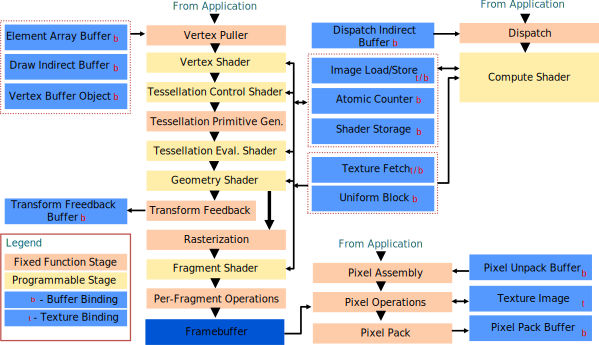
\includegraphics[width=11cm,keepaspectratio]{pics/opengl43.pdf}
	\end{figure}
\end{frame}


\begin{frame}
\frametitle{glBindBuffer() - hodnoty parametru target}
		\begin{description}
			\item[GL\_ARRAY\_BUFFER] Bufferu bude sloužit jako zdroj vrcholových dat
			\item[GL\_ELEMENT\_ARRAY\_BUFFER] Buffer bude sloužit jako indexy
			\item[GL\_ATOMIC\_COUNTER\_BUFFER] Buffer bude sloužit jako atomický čítač
			\item[GL\_DRAW\_INDIRECT\_BUFFER] Buffer bude sloužit pro indirect draw příkazy
			\item[...] ...
		\end{description}
\end{frame}

\begin{frame}[fragile]
\frametitle{Alokace Bufferu}
	\begin{itemize}

		\item{ Alokování bufferu - touto funkcí alokujeme buffer. Případně do něj můžeme nahrát data:\\
		{\scriptsize
		\begin{minted}[frame=lines]{c++}
		void glBufferData(GLenum target,GLsizeiptr size,
		                  const GLvoid*data,GLenum usage);
		\end{minted}
		}
		\begin{description}
			\item[target] Stejné jako u {\color{blue} glBindBuffer}.
			\item[size] Velikost bufferu v bajtech.
			\item[data] Ukazatel na data, která chceme nahrát.
			Při {\color{blue} NULL} se žádná data nekopírují.
			\item[usage] Způsob použití bufferu.
			Tímto parametrem sdělíme OpenGL, jakým způsobem budeme buffer používat.
			OpenGL zvolí nejvýhodnější alokaci bufferu z pohledu výkonnosti.
		\end{description}
		}

	\end{itemize}
\end{frame}

\begin{frame}
\frametitle{glBufferData() - hodnoty parametru usage}
	\begin{itemize}
		\item{Hodnoty GL\_X\_Y, kde X a Y je:}
		{\scriptsize
		\begin{tabular}{|l|l|}
		\hline
		X & popis \\ \hline
		STREAM & Data budou nahrána 1x a použita párkrát \\ \hline
		STATIC & Data budou nahrána 1x a použita mnohokrát \\ \hline
		DYNAMIC & Nahrání i používání dat bude časté \\ \hline
		\end{tabular}
		\begin{tabular}{|l|l|}
		\hline
		Y & popis \\ \hline
		DRAW & Data budou nahrána aplikací, vykreslení pomocí OpenGL \\ \hline
		READ & Data budou nahrána z OpenGL, aplikace čte data z VBO \\ \hline
		COPY & Data budou nahrána z OpenGL, vykreslení pomocí OpenGL \\ \hline
		\end{tabular}
		}
		\item{Hodnota parametru usage nijak neomezuje použití VBO.}
	\end{itemize}
\end{frame}

\begin{frame}[fragile]
\frametitle{Nahrání dat do Buffer}
	\begin{itemize}

		\item{ Funkcí pro alokaci dat můžeme také nahrát data.
		{\scriptsize
		\begin{minted}[frame=lines]{c++}
		void glBufferData(GLenum target,GLsizeiptr size,
		                  const GLvoid*data,GLenum usage);
		\end{minted}
		}}

		\item{ Nahrazení části bufferu novými daty.
		{\scriptsize
		\begin{minted}[frame=lines]{c++}
		void glBufferSubData(GLenum target,GLintptr offset,
		                     GLsizeiptr size,const GLvoid*data);
		\end{minted}
		}
		\begin{description}
		\item[target] Stejné jako u {\color{blue} glBindBuffer}.
		\item[offset] Offset v bajtech od začátku.
		\item[size] Velikost dat v bajtech
		\item[data] Ukazatel na data.
		\end{description}
		}
		{\scriptsize
		\begin{minted}[frame=lines]{c++}
		void glClearBufferData(GLenum target,GLenum internalformat,
		  GLenum format,GLenum type,const void * data);
		\end{minted}
		}
	\end{itemize}
\end{frame}

\begin{frame}[fragile]
\frametitle{Nahrání dat do Buffer}
	\begin{itemize}

		\item{ Touto funkcí můžeme 'vytáhnout' ukazatel na data v Bufferu.
		{\scriptsize
		\begin{minted}[frame=lines]{c++}
		void * glMapBuffer(GLenum target,GLenum access);
		\end{minted}
		}
		\begin{description}
		\item[target] Stejné jako u {\color{blue} glBindBuffer}.
		\item[access] Specifikuje přístup. Hodnoty GL\_READ\_ONLY, GL\_WRITE\_ONLY a GL\_READ\_WRITE.
		\end{description}
		}
		\item{ Po použití je potřeba uvolnit ukazatel.
		{\scriptsize
		\begin{minted}[frame=lines]{c++}
		GLboolean glUnmapBuffer(GLenum target);
		\end{minted}
		}}

	\end{itemize}
\end{frame}

\begin{frame}[fragile]
\frametitle{Příklad kódu}
	\begin{itemize}
		{\scriptsize
		\begin{minted}[frame=lines]{c++}
		float Data[]={0,0};//data, ktera budeme vkladat do bufferu
		GLuint VBO;//identifikator VBO
		glGenBuffers(1,&VBO);//vygenerujeme si identifikator
		glBindBuffer(GL_ARRAY_BUFFER,VBO);//aktivujeme si VBO
		//alokujeme buffer a nahrajeme do nej data
		glBufferData(GL_ARRAY_BUFFER,sizeof(Data),Data,GL_STATIC_DRAW);
		\end{minted}
		}
		Změna dat ve VBO.
		{\scriptsize
		\begin{minted}[frame=lines]{c++}
		float*ptr;//ukazatel na data
		ptr=(float*)glMapBuffer(GL_ARRAY_BUFFER,GL_READ_WRITE);//ziskame jej
		ptr[0]=0.5;//nastavime hodnotu prvniho prvku
		glUnmapBuffer(GL_ARRAY_BUFFER);//odmapujeme buffer
		\end{minted}
		}
		Nebo pomoci {\color{blue} glBufferSubData}.
		{\scriptsize
		\begin{minted}[frame=lines]{c++}
		glBufferSubData(GL_ARRAY_BUFFER,
		  sizeof(float),//nahrajeme nova s offsetem jeden float
		  sizeof(float),//nahrajeme jen jeden float
		  Data);//data
		\end{minted}
		}

	\end{itemize}
\end{frame}

\begin{frame}[fragile]
\frametitle{Vykreslení dat - získání identifikátoru atributu}
	\begin{itemize}
		\item{Vertex Shader:
		{\scriptsize
		\begin{minted}[frame=lines]{glsl}
		#version 330
		in vec2 inPos;//souradnice vertexu
		void main(){
		  gl_Position=vec4(inPos,0,1);
		}
		\end{minted}
		}}

		\item{Získání identifikátoru atributu z shaderu.
		{\scriptsize
		\begin{minted}[frame=lines]{c++}
		GLint inPosAttrib;//identifikator atributu
		inPosAttrib=glGetAttribLocation(
		  Shader,//shader program
		  "inPos");//nazev vstupni promenne v shaderu
		\end{minted}
		}}

	\end{itemize}
\end{frame}

\begin{frame}[fragile]
\frametitle{Vykreslení dat - navázání/aktivování atributu}
	\begin{itemize}
		\item{Před samotným vykreslením je potřeba navázat atributy na VBO.
		{\scriptsize
		\begin{minted}[frame=lines]{c++}
		void glVertexAttribPointer(GLuint index,GLint size,GLenum type,
		GLboolean normalized,GLsizei stride,const GLvoid * pointer);
		\end{minted}
		}
		\begin{description}
		\item[index] Identifikátor atributu získaný funkcí {\color{blue} glGetAttribLocation}
		\item[size] Počet komponent na atribut 1-4.
		\item[type] Datový typ GL\_FLOAT, GL\_INT, ...
		\item[normalized] normalizace GL\_FALSE, GL\_TRUE
		\item[stride] rozestup v bajtech
		\item[pointer] Offset v bajtech
		\end{description}
		}
		\item{Aktivování/deaktivování atributu
		{\scriptsize
		\begin{minted}[frame=lines]{c++}
		void glEnableVertexAttribArray(GLuint index);
		\end{minted}
		}
		{\scriptsize
		\begin{minted}[frame=lines]{c++}
		void glDisableVertexAttribArray(GLuint index);
		\end{minted}
		}}
	\end{itemize}
\end{frame}

\begin{frame}[fragile]
\frametitle{Navázání atributů k VBO Příklad (1)}
	\begin{itemize}
		\item{Předpokládejme, že budeme k jednomu vrcholu ukládat 4 atributy.
		Pozici (A), čas (B), barvu (C), texturovací koordináty (D).
		\begin{figure}[h]
		\includegraphics[width=10cm,keepaspectratio]{pics/stride.pdf}
		%\caption{Výpočet koeficinetu $a_2$}
		%\label{a2}
		\end{figure}
		}
	\end{itemize}
\end{frame}

\begin{frame}[fragile]
\frametitle{Navázání atributů k VBO Příklad (2)}
	\begin{itemize}
		\item{Shader program:
		{\scriptsize
		\begin{minted}[frame=lines]{glsl}
		#version 330
		in vec3 A;//souradnice vertexu
		in float B;//cas
		in vec3 C;//barva
		in vec2 D;//texturovaci koordinaty
		void main(){
			//...
		}
		\end{minted}
		}}

		\item{Aplikace:
		{\scriptsize
		\begin{minted}[frame=lines]{c++}
		GLint Aatt=glGetAttribLocation(Shader,"A");
		//...
		glEnableVertexAttribArray(Aattrib);
		//...
		glVertexAttribPointer(Aatt,3,GL_FLOAT,GL_FALSE,sizeof(float)*9,(GLvoid*)0);
		glVertexAttribPointer(Batt,1,GL_FLOAT,GL_FALSE,sizeof(float)*9,
		  (GLvoid*)(sizeof(float)*3));
		glVertexAttribPointer(Catt,3,GL_FLOAT,GL_FALSE,sizeof(float)*9,
		  (GLvoid*)(sizeof(float)*4));
		glVertexAttribPointer(Datt,2,GL_FLOAT,GL_FALSE,sizeof(float)*9,
		  (GLvoid*)(sizeof(float)*7));
		\end{minted}
		}}

	\end{itemize}
\end{frame}

\begin{frame}[fragile]
\frametitle{Vykreslení dat}
	\begin{itemize}
		\item{Data můžeme z VBO vykreslovat pomocí dvou způsobů - Přímo nebo indexovaně.}
		\item{Přímý způsob vykreslování:
		{\scriptsize
		\begin{minted}[frame=lines]{c++}
		void glDrawArrays(GLenum mode,GLint first,GLsizei count);
		\end{minted}
		}
		\begin{description}
		\item[mode] Typ primitiva: GL\_POINTS, GL\_LINE\_STRIP,GL\_LINE, ...
		\item[first] Počáteční index (první vrchol)
		\item[count] Počet indexů (počet vrcholů)
		\end{description}
		}
	\end{itemize}
\end{frame}

\begin{frame}[fragile]
\frametitle{Vykreslení dat}
	\begin{itemize}
		\item{Pro vykreslování s indexováním budeme potřebovat další buffer - Element buffer object (EBO). Buffer bude obsahovat indexy.
		{\scriptsize
		\begin{minted}[frame=lines]{c++}
		unsigned Data[]={0,1,1,3,0};//indexy
		GLuint EBO;//identifikator EBO
		glGenBuffers(1,&EBO);//vygenerujeme si identifikator
		glBindBuffer(GL_ELEMENT_ARRAY_BUFFER,EBO);//aktivujeme si EBO
		glBufferData(GL_ELEMENT_ARRAY_BUFFER,sizeof(Data),Data,GL_STATIC_DRAW);
		\end{minted}
		}}
		\item{Vykreslování s indexováním je vhodné například k ušetření místa - 
		několik polygonů sdílí stejný vrchol.
		}
		\item{ Kreslící funkce:
		{\scriptsize
		\begin{minted}[frame=lines]{c++}
		void glDrawElements(GLenum mode,GLsizei count,GLenum type,
		  const GLvoid * indices);
		\end{minted}
		}
		{\scriptsize
		\begin{minted}[frame=lines]{c++}
		void glDrawRangeElements(GLenum mode,GLuint start,GLuint end,
		  GLsizei count,GLenum type,const GLvoid * indices);
		\end{minted}
		}
		}
	\end{itemize}
\end{frame}

\begin{frame}[fragile]
\frametitle{glDrawElements()}
	\begin{itemize}
		{\scriptsize
		\begin{minted}[frame=lines]{c++}
		void glDrawElements(GLenum mode,GLsizei count,GLenum type,
		  const GLvoid * indices);
		\end{minted}
		}
		\begin{description}
		\item[mode] Typ vykreslovaného primitiva GL\_POINTS,GL\_LINES,...
		\item[count] Počet indexů (vrcholů), které chceme vykreslit.
		Pro jeden trojúhelník je toto číslo 3.
		\item[type] Typ indexu GL\_UNSIGNED\_BYTE, GL\_UNSIGNED\_SHORT, GL\_UNSIGNED\_INT.
		Čím menší typ zvolíme, tím bude kreslení rychlejší.
		\item[indices] Offset v bajtech - od kterého indexu se bude kreslit.
		\end{description}


	\end{itemize}
\end{frame}

\begin{frame}[fragile]
\frametitle{Kompletní příklad - shader}
		Vertex Shader:
		{\scriptsize
		\begin{minted}[frame=lines]{glsl}
		#version 330
		in vec2 vPos;//pozice
		in vec3 vCol;//barva vstup
		out vec3 fCol;//brava do fragment shaderu
		void main(){
		  gl_Position=vec4(vPos,0,1);
		  fCol=vCol;
		}
		\end{minted}
		}
		Fragment Shader:
		{\scriptsize
		\begin{minted}[frame=lines]{glsl}
		#version 330
		layout(location=0)out vec4 fragColor;//vystup
		in vec3 fCol;//barva
		void main(){
		  fragColor=vec4(fCol,1);
		}
		\end{minted}
		}
\end{frame}
%
\begin{frame}[fragile]
\frametitle{Kompletní příklad - aplikace}
		Aplikace - inicializace:
		{\scriptsize
		\begin{minted}[frame=lines]{c++}
		GLint vPos=glGetAttribLocation(Shader,"vPos");//ident. pozice
		GLint vCol=glGetAttribLocation(Shader,"vCol");//ident. barvy
		float Data[]={//pozice, barva
		   .0, .0,   1,0,1,
		  -.5, .5,   1,0,0,
		  -.5,-.5,   0,1,1,
		  -1,  .0,   1,0,0
		};
		glGenBuffers(1,&VBO);//jmeno pro VBO
		glBindBuffer(GL_ARRAY_BUFFER,VBO);//aktivujeme VBO
		glBufferData(GL_ARRAY_BUFFER,sizeof(Data),Data,GL_STATIC_DRAW);//data
		unsigned Index[]={0,1,2,2,1,3};//indexy
		glGenBuffers(1,&EBO);//jmeno pro EBO
		glBindBuffer(GL_ELEMENT_ARRAY_BUFFER,EBO);//aktivujeme EBO
		glBufferData(GL_ELEMENT_ARRAY_BUFFER,sizeof(Index),Index,GL_STATIC_DRAW);
		\end{minted}
		}
\end{frame}

\begin{frame}[fragile]
\frametitle{Kompletní příklad - aplikace}
		Aplikace - kreslení:
		{\scriptsize
		\begin{minted}[frame=lines]{c++}
		glBindBuffer(GL_ARRAY_BUFFER,VBO);//aktivujeme VBO
		glEnableVertexAttribArray(vPos);//aktivujeme vPos atribut
		glVertexAttribPointer(vPos,2,GL_FLOAT,GL_FALSE,sizeof(float)*5,
		  (GLvoid*)(sizeof(float)*0));//navazeme atribut na VBO

		glEnableVertexAttribArray(vCol);//aktivujeme vCol atribut
		glVertexAttribPointer(vCol,3,GL_FLOAT,GL_FALSE,sizeof(float)*5,
		  (GLvoid*)(sizeof(float)*2));//navazeme atribut na VBO

		glBindBuffer(GL_ELEMENT_ARRAY_BUFFER,EBO);//aktivujeme EBO
		glDrawElements(GL_TRIANGLES,6,GL_UNSIGNED_INT,NULL);//vykreslime
		\end{minted}
		}
\end{frame}

